%!TEX root = informe.tex
\chapter{Análisis de Ciclo de Vida: fabricación}
% Manual Euroadoquín. Documentos de Malaka.

\begin{figure}[!htb]
\centering
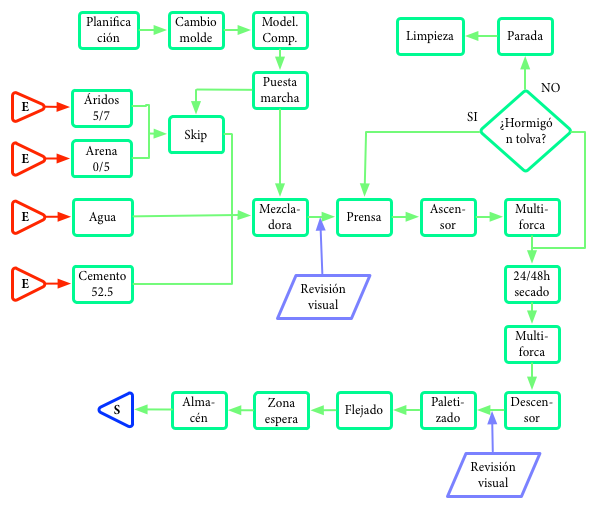
\includegraphics[width=15cm]{diagrama.png}
\caption{Diagrama de flujo de la fabricación de adoquines.}
\label{fig:diagrama_de_flujo}
\end{figure}

% \begin{figure}[!htb]
% \centering
% \begin{tikzpicture}[node distance=2cm]
% \node (start) [startstop] {Start};
% \node (in1) [io, below of=start] {Input};
% \node (pro1) [process, below of=in1] {Process 1};
% \node (dec1) [decision, below of=pro1, yshift=-0.5cm] {Decision 1};
% \node (pro2a) [process, below of=dec1, yshift=-1.5cm] {Process 2a text text text text text text text text text text};
% \node (pro2b) [process, right of=dec1, xshift=2cm] {Process 2b};
% \node (out1) [io, below of=pro2a] {Output};
% \node (stop) [startstop, below of=out1] {Stop};

% \draw [arrow] (start) -- (in1);
% \draw [arrow] (in1) -- (pro1);
% \draw [arrow] (pro1) -- (dec1);
% \draw [arrow] (dec1) -- node[anchor=east] {yes} (pro2a);
% \draw [arrow] (dec1) -- node[anchor=south] {no} (pro2b);
% \draw [arrow] (pro2b) |- (pro1);
% \draw [arrow] (pro2a) -- (out1);
% \draw [arrow] (out1) -- (stop);
% \end{tikzpicture}
% \caption{Prueba TikZ.}
% \label{fig:tikzpic}
% \end{figure}

\section{Cemento}
El cemento es transportado a granel en tanques a presión hasta la fábrica. Allí se almacena en silos previstos de compresores que descargan el material desde el tanque hasta su interior. El compresor es alimentado por electricidad mediante una toma de corriente conectada a la red eléctrica. El llenado a presión de los silos suele funcionar en rangos de 800—1000 \si{\cubic\meter/\minute} y presiones cercanas a 2 \si{\bar}, con potencias de 30 \si{\kilo\watt}. La descarga del silo, con una altura total de 20 \si{\meter}, es únicamente por gravedad con válvulas dosificadoras de control de caudal de hasta 35 \si{\tonne/\hour}.

\section{Arena y áridos}
Las arenas y áridos se transportan hasta la planta de fabricación mediante camiones. Actualmente los áridos y la arena ya no son apilados a bajo unos techados en las explanadas adyacentes a las plantas, sino que el propio transporte rellena las tolvas de forma automática.

Los áridos utilizados para producir adoquines puede incluir arena, gravilla y piedra de machaqueo si se pretende obtener un producto de peso normal. Si se desea que el adoquín sea más ligero —entre un 20 y un 45 \%— sin mermar sus propiedades estructurales se utilizan materiales como pizarra, arcilla, escoria de altos hornos y cenizas de carbón según su disponibilidad y coste.

\section{Agua}
El agua es muy importante en la constitución del hormigón. Reacciona químicamente con el cemento —hidratación— para proporcionar las propiedades deseadas del hormigón \cite{nrmca}. El agua de amasado es la cantidad de agua que toma contacto con el cemento y se usa para determinar las proporciones del resto de elementos para formar la mezcla. La fuerza y la durabilidad del cemento viene dado en gran parte por la cantidad de agua.

Además de su cantidad, la calidad del agua utilizada tiene efectos importantes en las propiedades del hormigón fresco, tales como el tiempo de graguado y la facilidad de trabajo. También tiene importantes en la fuerza y durabilidad del hormigón endurecido.

\subsection{Fuentes posibles de agua}

Por norma general el agua adecuada para el consumo humano —agua potable— es válida. No obstante, el agua no potable puede ser utilizada siempre que no tenga un impacto negativo en las propiedades del hormigón. La mayoría de las plantas tienen una fuente de agua municipal que proporciona potable sin pruebas de calidad. En zonas rurales o en plantas portátiles in situ —instaladas y desinstaladas en el propio lugar del proyecto—, habrá que utilizar fuentes de agua no potable como ríos o masas de agua.

Otra fuente de agua es la reciclada de la limpieza —agua de lavado— de la mezcladora y otros elementos de la planta. También se podrá aprovechar el agua de precipitaciones atmosféricas que pueda recolectarse en las instalaciones de la planta.

El agua de procesado no sólo se genera de la fabricación del hormigón, sino también del lavado del hormigón reciclado. Los sistemas de recolección procesan el agua con el cemento y los áridos en forma de lechada que puede ser también utilizada como agua para la mezcla de hormigón.

Las normativas medioambientales suelen requerir que las plantas de fabricación traten y procesen tanto el agua de lluvia como el de procesado —agua de operaciones— para que adquiera ciertos niveles de pH y contenidos sólidos antes de que abandonen las instalaciones \cite{ermco}.

\subsection{Cualificación del agua no potable}
El agua es el recurso más importante para el ser humano. En algunas zonas el suministro de agua potable es muy escaso. El uso de fuentes de agua no potables para la producción de hormigón mantiene una producción sostenible de hormigón conservando los recursos de agua potable. La gestión del agua procedente de la producción de hormigón conforme con las normativas medioambientales representa un coste adicional para el fabricante, por lo que el uso de agua no potable representa un ahorro considerable en la producción de hormigón. Cuando se utilizan fuentes de agua no potable es importante verificar y documentar que las impurezas que contiene no merman las características del hormigón, ya que las fuentes pueden contener aceites, grasas, sales disueltas y otros elementos no controlados. Por esta razón, el fabricante debería tener en cuenta que su uso implica un coste adicional que evaluar y controlar.

\section{Cintas transportadoras}

Las tolvas tienen dosificadores que descargan la cantidad programada de materia prima sobre dos cintas transportadoras —una para áridos y arena, otra para cemento— con básculas de pesaje incorporadas que se comunican con el sistema de control y cortan el flujo de descarga.

La cinta de áridos descarga sobre un skip que eleva los materiales hasta una mezcladora. La cinta de cemento descarga directamente sobre la mezcladora.Previamente al añadido del agua se produce un ciclo de mezclado en seco. Para asegurar la consistencia del lote el agua es generalmente añadido mediante un sistema electrónico de control que dosifica el caudal. En el caso de que haya otros aditivos, tales como acelerantes o colorantes, es en este momento cuando se incorporan a la mezcla. Cuando se termina de añadir el agua se produce el mezclado creando hormigón fresco. El hormigón sale de la mezcladora mediante una cinta transportadora que contiene otra báscula de pesaje y se dirige hacia la tolva de hormigón que se encuentra en lo alto de la prensa, donde es dosificado en los moldes para adoquines. Los moldes tienen una longevidad muy alta —aproximadamente un millón de ciclos de prensado— y su durabilidad depende de las propiedades abrasivas de los áridos utilizados.

El molde se compone de dos partes: la parte donde se inyecta el hormigón (hembra) y la parte que se coloca encima para dar forma (macho). La prensa tiene incorporado un carro alimentador encargado de proporcionar la parte hembra. Se inyecta el hormigón en el molde hembra, el molde macho baja con la prensa y el hormigón es compactado y cimentado usando un sistema combinado de presión y vibración. Cada molde puede producir 25 adoquines de 200x100x60\si{\milli\meter}, lo que proporciona a una superficie adoquinada de 0.5\si{\square\meter}. Los adoquines son moldeados de una sola pieza y extraidos del molde inmediatamente después de la vibro-compresión sobre una bandeja de madera.

La bandeja con las piezas frescas es trasladada sobre un transportador de rodillos hasta un ascensor. Este ascensor tiene diez alturas, de forma que cada vez que recibe una bandeja con adoquines frescos, la bandeja anterior sube una altura y monta la siguiente.

El ascensor se encarga de alimentar un carro multiforca de diez alturas. Cuando las diez alturas está ocupadas se cargan en un carro multiforca automatizado que transporta las piezas hasta un secadero.

Las piezas permanecen en el secadero curándose a temperatura ambiente entre 24 y 48 horas.

Una vez transcurrido el tiempo de curado, los adoquines están secos y listos para ser recogidos por otro carro multiforca automatizado que recoge las bandejas y las lleva a un descensor.

El descensor coloca las bandejas con los adoquines secos en un transportador de rodillos.

El transportador de rodillos lleva las bandejas hasta una paletizadora para hacer bloques de hasta cinco alturas.

La paletizadora impulsa el pallet hasta la flejadora que aplica varias lazadas de flejes para evitar que los adoquines se desprendan del conjunto.

La flejadora descansa los conjuntos paletizados sobre un un transportador de rodillos para ser posteriormente llevados a almacén.

Finalmente, un torito transporta cada conjunto de adoquines a la zona de almacenaje.


\section{Dosificación}
\section{Amasado}
\section{Vibrocompresión}
\section{Curado}
\section{Embalaje y almacenamiento}
\section{Suministro}
\section{Recepción}
